\documentclass[border=8pt]{standalone}
\usepackage[T1]{fontenc}\usepackage{lmodern}\usepackage{xspace}
\usepackage{amsmath,amssymb,amsfonts,mathtools}
\usepackage[table]{xcolor}\usepackage{graphicx}
\usepackage{tikz}\usetikzlibrary{arrows.meta,calc,fit,positioning,shapes,decorations.pathreplacing}
\setlength{\textwidth}{17cm}
% ── Colors used in the figures and tables ────────────────────────────────────
\definecolor{actcol}{HTML}{D32F2F}   % red: always active / restricted
\definecolor{arbcol}{HTML}{00A000}   % green: varying
\definecolor{parcol}{HTML}{0000FF}   % blue: parity
\colorlet{hilite}{black!12}          % one gray for everything the paper highlights

% ── Bit-index macros ─────────────────────────────────────────────────────────
% red italic = always active, green upright = varying, blue = parity,
% red box = punctured, plain black = no class.
\newcommand{\actbit}[1]{\textcolor{actcol}{\textit{#1}}}
\newcommand{\arbbit}[1]{\textcolor{arbcol}{#1}}
\newcommand{\parbit}[1]{\textcolor{parcol}{#1}}
% Robust, because it is used inside \caption, which is a moving argument.
\DeclareRobustCommand{\puncbit}[1]{\mbox{\tikz[baseline=(pb.base)]{%
  \node[draw=actcol, dashed, line width=0.5pt, rounded corners=1pt,
        inner xsep=1.6pt, inner ysep=1pt] (pb) {\ensuremath{#1}};}}}
\newcommand{\extbit}[1]{#1}                 % a bit entering a subround
\newcommand{\freebit}[1]{\parbit{#1}}       % a bit of the parity
\newcommand{\Pp}[1]{\actbit{#1}}
\newcommand{\Vv}[1]{\arbbit{#1}}

\newcommand{\CS}{2.6}
\newcommand{\PS}{11.9}
\newcommand{\RS}{17}   % row separation for the 2x2 subround panel figure
\tikzset{
  wire/.style  = {-{Latex[length=1.9mm,width=1.5mm]}, thick},
  % fig:forro-sr17-20 is two panels wide and fig:forro-sr17-22 three, so the
  % three-panel one is resized harder; the sizes below are the two-panel
  % defaults, and fig:forro-sr17-22 restates them larger to cancel that.
  rot/.style   = {draw, line width=0.7pt, rounded corners=1.2pt,
                  inner xsep=3pt, inner ysep=2.2pt,
                  font=\fontsize{13.1}{15}\selectfont},
  wname/.style = {font=\fontsize{10.9}{13}\selectfont},
  diff/.style  = {font=\fontsize{10.9}{13}\selectfont, align=center,
                  anchor=north, inner sep=1.5pt},
  title/.style = {font=\fontsize{9.1}{11}\selectfont\bfseries},
  % a word whose correlation-1 extension stops here: dashed red box + its f_i tag
  stopbox/.style = {draw=actcol, dashed, line width=0.5pt, rounded corners=1pt,
                    inner sep=2pt}
}
\newcommand{\srfops}{%
  % --- operators
  \node[opadd]  (dadd1) at ({3*\CS},-0.5) {};
  \node[opxor]  (cxor)  at ({2*\CS},-1.5) {};
  \node[opadd]  (badd)  at ({1*\CS},-2.5) {};
  \node[rot] (brot)  at ({1*\CS},-3.75) {$\lll 10$};
  \node[opadd]  (aadd1) at (0,-4.5) {};
  \node[opxor]  (exor)  at ({4*\CS},-5.2) {};
  \node[opadd]  (dadd2) at ({3*\CS},-6.0) {};
  \node[rot] (drot)  at ({3*\CS},-7.25) {$\lll 27$};
  \node[opadd]  (cadd)  at ({2*\CS},-8.0) {};
  \node[opxor]  (bxor)  at ({1*\CS},-9.0) {};
  \node[opadd]  (aadd2) at (0,-9.7) {};
  \node[rot] (arot)  at (0,-10.8)       {$\lll 8$};
  % --- vertical wires
  \draw[wire] (0,0.5) -- (aadd1);        \draw[wire] (aadd1) -- (aadd2);
  \draw[wire] (aadd2) -- (arot);         \draw[wire] (arot) -- (0,-11.7);
  \draw[wire] ({1*\CS},0.5) -- (badd);   \draw[wire] (badd) -- (brot);
  \draw[wire] (brot) -- (bxor);          \draw[wire] (bxor) -- ({1*\CS},-11.7);
  \draw[wire] ({2*\CS},0.5) -- (cxor);   \draw[wire] (cxor) -- (cadd);
  \draw[wire] (cadd) -- ({2*\CS},-11.7);
  \draw[wire] ({3*\CS},0.5) -- (dadd1);  \draw[wire] (dadd1) -- (dadd2);
  \draw[wire] (dadd2) -- (drot);         \draw[wire] (drot) -- ({3*\CS},-11.7);
  \draw[wire] ({4*\CS},0.5) -- (exor);   \draw[wire] (exor) -- ({4*\CS},-11.7);
  % --- horizontal taps (source wire -> operator)
  \draw[wire] ({4*\CS},-0.5)  -- (dadd1);   % d += e
  \draw[wire] ({3*\CS},-1.5)  -- (cxor);    % c ^= d
  \draw[wire] ({2*\CS},-2.5)  -- (badd);    % b += c
  \draw[wire] ({1*\CS},-4.5)  -- (aadd1);   % a += b
  \draw[wire] (0,-5.2)        -- (exor);    % e ^= a
  \draw[wire] ({4*\CS},-6.0)  -- (dadd2);   % d += e
  \draw[wire] ({3*\CS},-8.0)  -- (cadd);    % c += d
  \draw[wire] ({2*\CS},-9.0)  -- (bxor);    % b ^= c
  \draw[wire] ({1*\CS},-9.7) -- (aadd2);   % a += b
}
% top / bottom word names: #1..#5 = a,b,c,d,e
\newcommand{\srfin}[5]{%
  \node[wname] at (0,2) {$#1$};        \node[wname] at ({1*\CS},2) {$#2$};
  \node[wname] at ({2*\CS},2) {$#3$};  \node[wname] at ({3*\CS},2) {$#4$};
  \node[wname] at ({4*\CS},2) {$#5$};}
\newcommand{\srfout}[5]{%
  \node[wname] at (0,-12.15) {$#1$};       \node[wname] at ({1*\CS},-12.15) {$#2$};
  \node[wname] at ({2*\CS},-12.15) {$#3$}; \node[wname] at ({3*\CS},-12.15) {$#4$};
  \node[wname] at ({4*\CS},-12.15) {$#5$};}
% Mask carried in / out with correlation 1; $[\,]$ = nothing on that word.
% Nodes are named ia..ie / oa..oe so that \stopbit can box one of them.
\newcommand{\srfdiffin}[5]{%
  \node[diff] (ia) at (0,1.6) {#1};       \node[diff] (ib) at ({1*\CS},1.6) {#2};
  \node[diff] (ic) at ({2*\CS},1.6) {#3}; \node[diff] (id) at ({3*\CS},1.6) {#4};
  \node[diff] (ie) at ({4*\CS},1.6) {#5};}
\newcommand{\srfdiffout}[5]{%
  \node[diff] (oa) at (0,-12.5) {#1};       \node[diff] (ob) at ({1*\CS},-12.5) {#2};
  \node[diff] (oc) at ({2*\CS},-12.5) {#3}; \node[diff] (od) at ({3*\CS},-12.5) {#4};
  \node[diff] (oe) at ({4*\CS},-12.5) {#5};}
% \stopbit{node}{tag}: put the red puncturing box round the bit whose
% correlation-1 extension stops here, and tag it with the function it is
% punctured into, e.g. \stopbit{id}{f_1}
\newcommand{\stopbit}[2]{%
  \node[stopbox, fit=(#1)] {};
  \node[font=\scriptsize, text=actcol, anchor=north] at ($(#1.south)+(0,-0.12)$) {$#2$};}

% ── CPNB figure palette ──────────────────────────────────────────────────────
% Four fills whose lightness is well separated, so the classification survives
% black and white printing: white 100%, cpnbcol 80%, synccol 49%, restcol 26%.
% restcol is actcol darkened, so a restricted bit reads as the same red as an
% always-active bit while keeping the lightness gap these figures rely on.
\definecolor{cpnbcol}{RGB}{204,204,204}
\definecolor{synccol}{RGB}{90,125,205}
\colorlet{restcol}{actcol!70!black}

% ── Uniform figure frame ─────────────────────────────────────────────────────
% Every figure is resized to the same stated width and gets the same padding,
% whatever scale factor that figure uses. The rule is set to zero width: the
% figures are not boxed, and a visible frame would compete with the dashed red
% box, which is the one frame in this paper that carries a meaning.
% #1 is the total width of the framed result, rule and padding included.
\newlength{\figframewidth}
\newcommand{\figframe}[2]{%
  \begingroup
  \setlength{\fboxrule}{0pt}%
  \setlength{\fboxsep}{12pt}%
  \setlength{\figframewidth}{#1}%
  \addtolength{\figframewidth}{-2\fboxsep}%
  \addtolength{\figframewidth}{-2\fboxrule}%
  \fbox{\resizebox{\figframewidth}{!}{#2}}%
  \endgroup}

% ── ARX operators ────────────────────────────────────────────────────────────
% The shape carries the meaning, so the figures read correctly without colour:
% square for addition modulo $2^{32}$, circle for XOR, rounded box for
% rotation.
% Operator geometry. Defaults suit the two-panel figures; a figure that is
% resized harder or softer resets these so the printed size stays the same.
\newlength{\opsize}\setlength{\opsize}{6mm}
\newlength{\oprule}\setlength{\oprule}{0.7pt}
\tikzset{
  % modular addition: a cross across a square, i.e. $\boxplus$
  opadd/.style = {draw, line width=\oprule, rectangle, minimum size=\opsize,
                  inner sep=0pt,
                  path picture={%
                    \draw[line width=\oprule]
                      (path picture bounding box.west) --
                      (path picture bounding box.east)
                      (path picture bounding box.south) --
                      (path picture bounding box.north);}},
  % rotation: a rounded box, so that it reads as an operator alongside the
  % square addition and the round XOR without being mistaken for either
  oprot/.style = {draw, line width=\oprule, rounded corners=1.2pt,
                  minimum height=\opsize, inner xsep=3pt, inner ysep=2.2pt,
                  font=\Large},
  % XOR: a cross running the full diameter of a circle, i.e. $\oplus$
  opxor/.style = {draw, line width=\oprule, circle, minimum size=\opsize,
                  inner sep=0pt,
                  path picture={%
                    \draw[line width=\oprule]
                      (path picture bounding box.west) --
                      (path picture bounding box.east)
                      (path picture bounding box.south) --
                      (path picture bounding box.north);}}
}

% ── Differential-linear arrow ────────────────────────────────────────────────
% One spelling for every distinguisher in the paper: \dlarrow{4} etc.
\newcommand{\dlarrow}[1]{%
  \underset{\text{#1 rounds}}{\overset{\mathcal{DL}}{\longrightarrow}}}

% ── Cipher name ─────────────────────────────────────────────────────────────
\newcommand{\Forro}{Forr\'o\xspace}


\begin{document}
\begin{minipage}{0.95\textwidth}\centering

\figframe{0.95\textwidth}{%
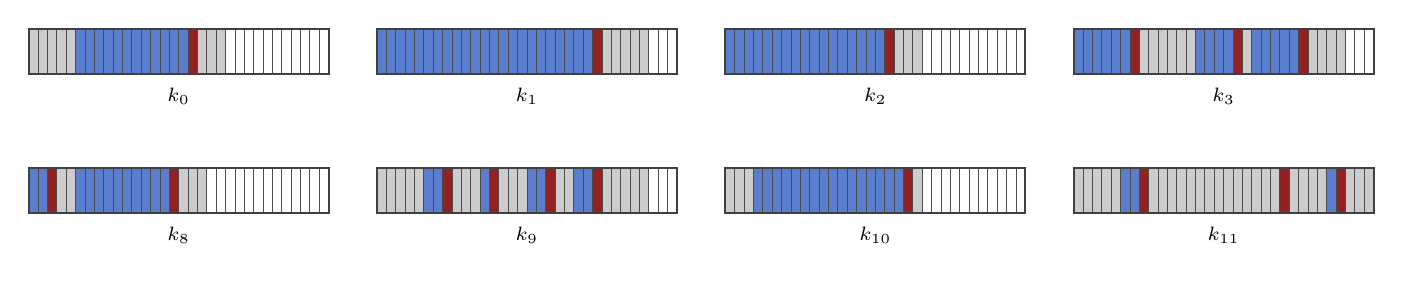
\begin{tikzpicture}[x=1.92cm,y=1.92cm,
    bit/.style={draw=black!70, line width=0.3pt},
    word/.style={draw=black!75, line width=0.75pt},
    every node/.style={font=\scriptsize}]
\filldraw[bit, fill=white] (1.922,0.000) rectangle (1.984,-0.300);
\filldraw[bit, fill=white] (1.860,0.000) rectangle (1.922,-0.300);
\filldraw[bit, fill=white] (1.798,0.000) rectangle (1.860,-0.300);
\filldraw[bit, fill=white] (1.736,0.000) rectangle (1.798,-0.300);
\filldraw[bit, fill=white] (1.674,0.000) rectangle (1.736,-0.300);
\filldraw[bit, fill=white] (1.612,0.000) rectangle (1.674,-0.300);
\filldraw[bit, fill=white] (1.550,0.000) rectangle (1.612,-0.300);
\filldraw[bit, fill=white] (1.488,0.000) rectangle (1.550,-0.300);
\filldraw[bit, fill=white] (1.426,0.000) rectangle (1.488,-0.300);
\filldraw[bit, fill=white] (1.364,0.000) rectangle (1.426,-0.300);
\filldraw[bit, fill=white] (1.302,0.000) rectangle (1.364,-0.300);
\filldraw[bit, fill=cpnbcol] (1.240,0.000) rectangle (1.302,-0.300);
\filldraw[bit, fill=cpnbcol] (1.178,0.000) rectangle (1.240,-0.300);
\filldraw[bit, fill=cpnbcol] (1.116,0.000) rectangle (1.178,-0.300);
\filldraw[bit, fill=restcol] (1.054,0.000) rectangle (1.116,-0.300);
\filldraw[bit, fill=synccol] (0.992,0.000) rectangle (1.054,-0.300);
\filldraw[bit, fill=synccol] (0.930,0.000) rectangle (0.992,-0.300);
\filldraw[bit, fill=synccol] (0.868,0.000) rectangle (0.930,-0.300);
\filldraw[bit, fill=synccol] (0.806,0.000) rectangle (0.868,-0.300);
\filldraw[bit, fill=synccol] (0.744,0.000) rectangle (0.806,-0.300);
\filldraw[bit, fill=synccol] (0.682,0.000) rectangle (0.744,-0.300);
\filldraw[bit, fill=synccol] (0.620,0.000) rectangle (0.682,-0.300);
\filldraw[bit, fill=synccol] (0.558,0.000) rectangle (0.620,-0.300);
\filldraw[bit, fill=synccol] (0.496,0.000) rectangle (0.558,-0.300);
\filldraw[bit, fill=synccol] (0.434,0.000) rectangle (0.496,-0.300);
\filldraw[bit, fill=synccol] (0.372,0.000) rectangle (0.434,-0.300);
\filldraw[bit, fill=synccol] (0.310,0.000) rectangle (0.372,-0.300);
\filldraw[bit, fill=cpnbcol] (0.248,0.000) rectangle (0.310,-0.300);
\filldraw[bit, fill=cpnbcol] (0.186,0.000) rectangle (0.248,-0.300);
\filldraw[bit, fill=cpnbcol] (0.124,0.000) rectangle (0.186,-0.300);
\filldraw[bit, fill=cpnbcol] (0.062,0.000) rectangle (0.124,-0.300);
\filldraw[bit, fill=cpnbcol] (0.000,0.000) rectangle (0.062,-0.300);
\draw[word] (0.000,0.000) rectangle (1.984,-0.300);
\node[anchor=north,font=\scriptsize] at (0.992,-0.330) {$k_{0}$};
\filldraw[bit, fill=white] (4.226,0.000) rectangle (4.288,-0.300);
\filldraw[bit, fill=white] (4.164,0.000) rectangle (4.226,-0.300);
\filldraw[bit, fill=white] (4.102,0.000) rectangle (4.164,-0.300);
\filldraw[bit, fill=cpnbcol] (4.040,0.000) rectangle (4.102,-0.300);
\filldraw[bit, fill=cpnbcol] (3.978,0.000) rectangle (4.040,-0.300);
\filldraw[bit, fill=cpnbcol] (3.916,0.000) rectangle (3.978,-0.300);
\filldraw[bit, fill=cpnbcol] (3.854,0.000) rectangle (3.916,-0.300);
\filldraw[bit, fill=cpnbcol] (3.792,0.000) rectangle (3.854,-0.300);
\filldraw[bit, fill=restcol] (3.730,0.000) rectangle (3.792,-0.300);
\filldraw[bit, fill=synccol] (3.668,0.000) rectangle (3.730,-0.300);
\filldraw[bit, fill=synccol] (3.606,0.000) rectangle (3.668,-0.300);
\filldraw[bit, fill=synccol] (3.544,0.000) rectangle (3.606,-0.300);
\filldraw[bit, fill=synccol] (3.482,0.000) rectangle (3.544,-0.300);
\filldraw[bit, fill=synccol] (3.420,0.000) rectangle (3.482,-0.300);
\filldraw[bit, fill=synccol] (3.358,0.000) rectangle (3.420,-0.300);
\filldraw[bit, fill=synccol] (3.296,0.000) rectangle (3.358,-0.300);
\filldraw[bit, fill=synccol] (3.234,0.000) rectangle (3.296,-0.300);
\filldraw[bit, fill=synccol] (3.172,0.000) rectangle (3.234,-0.300);
\filldraw[bit, fill=synccol] (3.110,0.000) rectangle (3.172,-0.300);
\filldraw[bit, fill=synccol] (3.048,0.000) rectangle (3.110,-0.300);
\filldraw[bit, fill=synccol] (2.986,0.000) rectangle (3.048,-0.300);
\filldraw[bit, fill=synccol] (2.924,0.000) rectangle (2.986,-0.300);
\filldraw[bit, fill=synccol] (2.862,0.000) rectangle (2.924,-0.300);
\filldraw[bit, fill=synccol] (2.800,0.000) rectangle (2.862,-0.300);
\filldraw[bit, fill=synccol] (2.738,0.000) rectangle (2.800,-0.300);
\filldraw[bit, fill=synccol] (2.676,0.000) rectangle (2.738,-0.300);
\filldraw[bit, fill=synccol] (2.614,0.000) rectangle (2.676,-0.300);
\filldraw[bit, fill=synccol] (2.552,0.000) rectangle (2.614,-0.300);
\filldraw[bit, fill=synccol] (2.490,0.000) rectangle (2.552,-0.300);
\filldraw[bit, fill=synccol] (2.428,0.000) rectangle (2.490,-0.300);
\filldraw[bit, fill=synccol] (2.366,0.000) rectangle (2.428,-0.300);
\filldraw[bit, fill=synccol] (2.304,0.000) rectangle (2.366,-0.300);
\draw[word] (2.304,0.000) rectangle (4.288,-0.300);
\node[anchor=north,font=\scriptsize] at (3.296,-0.330) {$k_{1}$};
\filldraw[bit, fill=white] (6.530,0.000) rectangle (6.592,-0.300);
\filldraw[bit, fill=white] (6.468,0.000) rectangle (6.530,-0.300);
\filldraw[bit, fill=white] (6.406,0.000) rectangle (6.468,-0.300);
\filldraw[bit, fill=white] (6.344,0.000) rectangle (6.406,-0.300);
\filldraw[bit, fill=white] (6.282,0.000) rectangle (6.344,-0.300);
\filldraw[bit, fill=white] (6.220,0.000) rectangle (6.282,-0.300);
\filldraw[bit, fill=white] (6.158,0.000) rectangle (6.220,-0.300);
\filldraw[bit, fill=white] (6.096,0.000) rectangle (6.158,-0.300);
\filldraw[bit, fill=white] (6.034,0.000) rectangle (6.096,-0.300);
\filldraw[bit, fill=white] (5.972,0.000) rectangle (6.034,-0.300);
\filldraw[bit, fill=white] (5.910,0.000) rectangle (5.972,-0.300);
\filldraw[bit, fill=cpnbcol] (5.848,0.000) rectangle (5.910,-0.300);
\filldraw[bit, fill=cpnbcol] (5.786,0.000) rectangle (5.848,-0.300);
\filldraw[bit, fill=cpnbcol] (5.724,0.000) rectangle (5.786,-0.300);
\filldraw[bit, fill=restcol] (5.662,0.000) rectangle (5.724,-0.300);
\filldraw[bit, fill=synccol] (5.600,0.000) rectangle (5.662,-0.300);
\filldraw[bit, fill=synccol] (5.538,0.000) rectangle (5.600,-0.300);
\filldraw[bit, fill=synccol] (5.476,0.000) rectangle (5.538,-0.300);
\filldraw[bit, fill=synccol] (5.414,0.000) rectangle (5.476,-0.300);
\filldraw[bit, fill=synccol] (5.352,0.000) rectangle (5.414,-0.300);
\filldraw[bit, fill=synccol] (5.290,0.000) rectangle (5.352,-0.300);
\filldraw[bit, fill=synccol] (5.228,0.000) rectangle (5.290,-0.300);
\filldraw[bit, fill=synccol] (5.166,0.000) rectangle (5.228,-0.300);
\filldraw[bit, fill=synccol] (5.104,0.000) rectangle (5.166,-0.300);
\filldraw[bit, fill=synccol] (5.042,0.000) rectangle (5.104,-0.300);
\filldraw[bit, fill=synccol] (4.980,0.000) rectangle (5.042,-0.300);
\filldraw[bit, fill=synccol] (4.918,0.000) rectangle (4.980,-0.300);
\filldraw[bit, fill=synccol] (4.856,0.000) rectangle (4.918,-0.300);
\filldraw[bit, fill=synccol] (4.794,0.000) rectangle (4.856,-0.300);
\filldraw[bit, fill=synccol] (4.732,0.000) rectangle (4.794,-0.300);
\filldraw[bit, fill=synccol] (4.670,0.000) rectangle (4.732,-0.300);
\filldraw[bit, fill=synccol] (4.608,0.000) rectangle (4.670,-0.300);
\draw[word] (4.608,0.000) rectangle (6.592,-0.300);
\node[anchor=north,font=\scriptsize] at (5.600,-0.330) {$k_{2}$};
\filldraw[bit, fill=white] (8.834,0.000) rectangle (8.896,-0.300);
\filldraw[bit, fill=white] (8.772,0.000) rectangle (8.834,-0.300);
\filldraw[bit, fill=white] (8.710,0.000) rectangle (8.772,-0.300);
\filldraw[bit, fill=cpnbcol] (8.648,0.000) rectangle (8.710,-0.300);
\filldraw[bit, fill=cpnbcol] (8.586,0.000) rectangle (8.648,-0.300);
\filldraw[bit, fill=cpnbcol] (8.524,0.000) rectangle (8.586,-0.300);
\filldraw[bit, fill=cpnbcol] (8.462,0.000) rectangle (8.524,-0.300);
\filldraw[bit, fill=restcol] (8.400,0.000) rectangle (8.462,-0.300);
\filldraw[bit, fill=synccol] (8.338,0.000) rectangle (8.400,-0.300);
\filldraw[bit, fill=synccol] (8.276,0.000) rectangle (8.338,-0.300);
\filldraw[bit, fill=synccol] (8.214,0.000) rectangle (8.276,-0.300);
\filldraw[bit, fill=synccol] (8.152,0.000) rectangle (8.214,-0.300);
\filldraw[bit, fill=synccol] (8.090,0.000) rectangle (8.152,-0.300);
\filldraw[bit, fill=cpnbcol] (8.028,0.000) rectangle (8.090,-0.300);
\filldraw[bit, fill=restcol] (7.966,0.000) rectangle (8.028,-0.300);
\filldraw[bit, fill=synccol] (7.904,0.000) rectangle (7.966,-0.300);
\filldraw[bit, fill=synccol] (7.842,0.000) rectangle (7.904,-0.300);
\filldraw[bit, fill=synccol] (7.780,0.000) rectangle (7.842,-0.300);
\filldraw[bit, fill=synccol] (7.718,0.000) rectangle (7.780,-0.300);
\filldraw[bit, fill=cpnbcol] (7.656,0.000) rectangle (7.718,-0.300);
\filldraw[bit, fill=cpnbcol] (7.594,0.000) rectangle (7.656,-0.300);
\filldraw[bit, fill=cpnbcol] (7.532,0.000) rectangle (7.594,-0.300);
\filldraw[bit, fill=cpnbcol] (7.470,0.000) rectangle (7.532,-0.300);
\filldraw[bit, fill=cpnbcol] (7.408,0.000) rectangle (7.470,-0.300);
\filldraw[bit, fill=cpnbcol] (7.346,0.000) rectangle (7.408,-0.300);
\filldraw[bit, fill=restcol] (7.284,0.000) rectangle (7.346,-0.300);
\filldraw[bit, fill=synccol] (7.222,0.000) rectangle (7.284,-0.300);
\filldraw[bit, fill=synccol] (7.160,0.000) rectangle (7.222,-0.300);
\filldraw[bit, fill=synccol] (7.098,0.000) rectangle (7.160,-0.300);
\filldraw[bit, fill=synccol] (7.036,0.000) rectangle (7.098,-0.300);
\filldraw[bit, fill=synccol] (6.974,0.000) rectangle (7.036,-0.300);
\filldraw[bit, fill=synccol] (6.912,0.000) rectangle (6.974,-0.300);
\draw[word] (6.912,0.000) rectangle (8.896,-0.300);
\node[anchor=north,font=\scriptsize] at (7.904,-0.330) {$k_{3}$};
\filldraw[bit, fill=white] (1.922,-0.920) rectangle (1.984,-1.220);
\filldraw[bit, fill=white] (1.860,-0.920) rectangle (1.922,-1.220);
\filldraw[bit, fill=white] (1.798,-0.920) rectangle (1.860,-1.220);
\filldraw[bit, fill=white] (1.736,-0.920) rectangle (1.798,-1.220);
\filldraw[bit, fill=white] (1.674,-0.920) rectangle (1.736,-1.220);
\filldraw[bit, fill=white] (1.612,-0.920) rectangle (1.674,-1.220);
\filldraw[bit, fill=white] (1.550,-0.920) rectangle (1.612,-1.220);
\filldraw[bit, fill=white] (1.488,-0.920) rectangle (1.550,-1.220);
\filldraw[bit, fill=white] (1.426,-0.920) rectangle (1.488,-1.220);
\filldraw[bit, fill=white] (1.364,-0.920) rectangle (1.426,-1.220);
\filldraw[bit, fill=white] (1.302,-0.920) rectangle (1.364,-1.220);
\filldraw[bit, fill=white] (1.240,-0.920) rectangle (1.302,-1.220);
\filldraw[bit, fill=white] (1.178,-0.920) rectangle (1.240,-1.220);
\filldraw[bit, fill=cpnbcol] (1.116,-0.920) rectangle (1.178,-1.220);
\filldraw[bit, fill=cpnbcol] (1.054,-0.920) rectangle (1.116,-1.220);
\filldraw[bit, fill=cpnbcol] (0.992,-0.920) rectangle (1.054,-1.220);
\filldraw[bit, fill=restcol] (0.930,-0.920) rectangle (0.992,-1.220);
\filldraw[bit, fill=synccol] (0.868,-0.920) rectangle (0.930,-1.220);
\filldraw[bit, fill=synccol] (0.806,-0.920) rectangle (0.868,-1.220);
\filldraw[bit, fill=synccol] (0.744,-0.920) rectangle (0.806,-1.220);
\filldraw[bit, fill=synccol] (0.682,-0.920) rectangle (0.744,-1.220);
\filldraw[bit, fill=synccol] (0.620,-0.920) rectangle (0.682,-1.220);
\filldraw[bit, fill=synccol] (0.558,-0.920) rectangle (0.620,-1.220);
\filldraw[bit, fill=synccol] (0.496,-0.920) rectangle (0.558,-1.220);
\filldraw[bit, fill=synccol] (0.434,-0.920) rectangle (0.496,-1.220);
\filldraw[bit, fill=synccol] (0.372,-0.920) rectangle (0.434,-1.220);
\filldraw[bit, fill=synccol] (0.310,-0.920) rectangle (0.372,-1.220);
\filldraw[bit, fill=cpnbcol] (0.248,-0.920) rectangle (0.310,-1.220);
\filldraw[bit, fill=cpnbcol] (0.186,-0.920) rectangle (0.248,-1.220);
\filldraw[bit, fill=restcol] (0.124,-0.920) rectangle (0.186,-1.220);
\filldraw[bit, fill=synccol] (0.062,-0.920) rectangle (0.124,-1.220);
\filldraw[bit, fill=synccol] (0.000,-0.920) rectangle (0.062,-1.220);
\draw[word] (0.000,-0.920) rectangle (1.984,-1.220);
\node[anchor=north,font=\scriptsize] at (0.992,-1.250) {$k_{8}$};
\filldraw[bit, fill=white] (4.226,-0.920) rectangle (4.288,-1.220);
\filldraw[bit, fill=white] (4.164,-0.920) rectangle (4.226,-1.220);
\filldraw[bit, fill=white] (4.102,-0.920) rectangle (4.164,-1.220);
\filldraw[bit, fill=cpnbcol] (4.040,-0.920) rectangle (4.102,-1.220);
\filldraw[bit, fill=cpnbcol] (3.978,-0.920) rectangle (4.040,-1.220);
\filldraw[bit, fill=cpnbcol] (3.916,-0.920) rectangle (3.978,-1.220);
\filldraw[bit, fill=cpnbcol] (3.854,-0.920) rectangle (3.916,-1.220);
\filldraw[bit, fill=cpnbcol] (3.792,-0.920) rectangle (3.854,-1.220);
\filldraw[bit, fill=restcol] (3.730,-0.920) rectangle (3.792,-1.220);
\filldraw[bit, fill=synccol] (3.668,-0.920) rectangle (3.730,-1.220);
\filldraw[bit, fill=synccol] (3.606,-0.920) rectangle (3.668,-1.220);
\filldraw[bit, fill=cpnbcol] (3.544,-0.920) rectangle (3.606,-1.220);
\filldraw[bit, fill=cpnbcol] (3.482,-0.920) rectangle (3.544,-1.220);
\filldraw[bit, fill=restcol] (3.420,-0.920) rectangle (3.482,-1.220);
\filldraw[bit, fill=synccol] (3.358,-0.920) rectangle (3.420,-1.220);
\filldraw[bit, fill=synccol] (3.296,-0.920) rectangle (3.358,-1.220);
\filldraw[bit, fill=cpnbcol] (3.234,-0.920) rectangle (3.296,-1.220);
\filldraw[bit, fill=cpnbcol] (3.172,-0.920) rectangle (3.234,-1.220);
\filldraw[bit, fill=cpnbcol] (3.110,-0.920) rectangle (3.172,-1.220);
\filldraw[bit, fill=restcol] (3.048,-0.920) rectangle (3.110,-1.220);
\filldraw[bit, fill=synccol] (2.986,-0.920) rectangle (3.048,-1.220);
\filldraw[bit, fill=cpnbcol] (2.924,-0.920) rectangle (2.986,-1.220);
\filldraw[bit, fill=cpnbcol] (2.862,-0.920) rectangle (2.924,-1.220);
\filldraw[bit, fill=cpnbcol] (2.800,-0.920) rectangle (2.862,-1.220);
\filldraw[bit, fill=restcol] (2.738,-0.920) rectangle (2.800,-1.220);
\filldraw[bit, fill=synccol] (2.676,-0.920) rectangle (2.738,-1.220);
\filldraw[bit, fill=synccol] (2.614,-0.920) rectangle (2.676,-1.220);
\filldraw[bit, fill=cpnbcol] (2.552,-0.920) rectangle (2.614,-1.220);
\filldraw[bit, fill=cpnbcol] (2.490,-0.920) rectangle (2.552,-1.220);
\filldraw[bit, fill=cpnbcol] (2.428,-0.920) rectangle (2.490,-1.220);
\filldraw[bit, fill=cpnbcol] (2.366,-0.920) rectangle (2.428,-1.220);
\filldraw[bit, fill=cpnbcol] (2.304,-0.920) rectangle (2.366,-1.220);
\draw[word] (2.304,-0.920) rectangle (4.288,-1.220);
\node[anchor=north,font=\scriptsize] at (3.296,-1.250) {$k_{9}$};
\filldraw[bit, fill=white] (6.530,-0.920) rectangle (6.592,-1.220);
\filldraw[bit, fill=white] (6.468,-0.920) rectangle (6.530,-1.220);
\filldraw[bit, fill=white] (6.406,-0.920) rectangle (6.468,-1.220);
\filldraw[bit, fill=white] (6.344,-0.920) rectangle (6.406,-1.220);
\filldraw[bit, fill=white] (6.282,-0.920) rectangle (6.344,-1.220);
\filldraw[bit, fill=white] (6.220,-0.920) rectangle (6.282,-1.220);
\filldraw[bit, fill=white] (6.158,-0.920) rectangle (6.220,-1.220);
\filldraw[bit, fill=white] (6.096,-0.920) rectangle (6.158,-1.220);
\filldraw[bit, fill=white] (6.034,-0.920) rectangle (6.096,-1.220);
\filldraw[bit, fill=white] (5.972,-0.920) rectangle (6.034,-1.220);
\filldraw[bit, fill=white] (5.910,-0.920) rectangle (5.972,-1.220);
\filldraw[bit, fill=cpnbcol] (5.848,-0.920) rectangle (5.910,-1.220);
\filldraw[bit, fill=restcol] (5.786,-0.920) rectangle (5.848,-1.220);
\filldraw[bit, fill=synccol] (5.724,-0.920) rectangle (5.786,-1.220);
\filldraw[bit, fill=synccol] (5.662,-0.920) rectangle (5.724,-1.220);
\filldraw[bit, fill=synccol] (5.600,-0.920) rectangle (5.662,-1.220);
\filldraw[bit, fill=synccol] (5.538,-0.920) rectangle (5.600,-1.220);
\filldraw[bit, fill=synccol] (5.476,-0.920) rectangle (5.538,-1.220);
\filldraw[bit, fill=synccol] (5.414,-0.920) rectangle (5.476,-1.220);
\filldraw[bit, fill=synccol] (5.352,-0.920) rectangle (5.414,-1.220);
\filldraw[bit, fill=synccol] (5.290,-0.920) rectangle (5.352,-1.220);
\filldraw[bit, fill=synccol] (5.228,-0.920) rectangle (5.290,-1.220);
\filldraw[bit, fill=synccol] (5.166,-0.920) rectangle (5.228,-1.220);
\filldraw[bit, fill=synccol] (5.104,-0.920) rectangle (5.166,-1.220);
\filldraw[bit, fill=synccol] (5.042,-0.920) rectangle (5.104,-1.220);
\filldraw[bit, fill=synccol] (4.980,-0.920) rectangle (5.042,-1.220);
\filldraw[bit, fill=synccol] (4.918,-0.920) rectangle (4.980,-1.220);
\filldraw[bit, fill=synccol] (4.856,-0.920) rectangle (4.918,-1.220);
\filldraw[bit, fill=synccol] (4.794,-0.920) rectangle (4.856,-1.220);
\filldraw[bit, fill=cpnbcol] (4.732,-0.920) rectangle (4.794,-1.220);
\filldraw[bit, fill=cpnbcol] (4.670,-0.920) rectangle (4.732,-1.220);
\filldraw[bit, fill=cpnbcol] (4.608,-0.920) rectangle (4.670,-1.220);
\draw[word] (4.608,-0.920) rectangle (6.592,-1.220);
\node[anchor=north,font=\scriptsize] at (5.600,-1.250) {$k_{10}$};
\filldraw[bit, fill=cpnbcol] (8.834,-0.920) rectangle (8.896,-1.220);
\filldraw[bit, fill=cpnbcol] (8.772,-0.920) rectangle (8.834,-1.220);
\filldraw[bit, fill=cpnbcol] (8.710,-0.920) rectangle (8.772,-1.220);
\filldraw[bit, fill=restcol] (8.648,-0.920) rectangle (8.710,-1.220);
\filldraw[bit, fill=synccol] (8.586,-0.920) rectangle (8.648,-1.220);
\filldraw[bit, fill=cpnbcol] (8.524,-0.920) rectangle (8.586,-1.220);
\filldraw[bit, fill=cpnbcol] (8.462,-0.920) rectangle (8.524,-1.220);
\filldraw[bit, fill=cpnbcol] (8.400,-0.920) rectangle (8.462,-1.220);
\filldraw[bit, fill=cpnbcol] (8.338,-0.920) rectangle (8.400,-1.220);
\filldraw[bit, fill=restcol] (8.276,-0.920) rectangle (8.338,-1.220);
\filldraw[bit, fill=cpnbcol] (8.214,-0.920) rectangle (8.276,-1.220);
\filldraw[bit, fill=cpnbcol] (8.152,-0.920) rectangle (8.214,-1.220);
\filldraw[bit, fill=cpnbcol] (8.090,-0.920) rectangle (8.152,-1.220);
\filldraw[bit, fill=cpnbcol] (8.028,-0.920) rectangle (8.090,-1.220);
\filldraw[bit, fill=cpnbcol] (7.966,-0.920) rectangle (8.028,-1.220);
\filldraw[bit, fill=cpnbcol] (7.904,-0.920) rectangle (7.966,-1.220);
\filldraw[bit, fill=cpnbcol] (7.842,-0.920) rectangle (7.904,-1.220);
\filldraw[bit, fill=cpnbcol] (7.780,-0.920) rectangle (7.842,-1.220);
\filldraw[bit, fill=cpnbcol] (7.718,-0.920) rectangle (7.780,-1.220);
\filldraw[bit, fill=cpnbcol] (7.656,-0.920) rectangle (7.718,-1.220);
\filldraw[bit, fill=cpnbcol] (7.594,-0.920) rectangle (7.656,-1.220);
\filldraw[bit, fill=cpnbcol] (7.532,-0.920) rectangle (7.594,-1.220);
\filldraw[bit, fill=cpnbcol] (7.470,-0.920) rectangle (7.532,-1.220);
\filldraw[bit, fill=cpnbcol] (7.408,-0.920) rectangle (7.470,-1.220);
\filldraw[bit, fill=restcol] (7.346,-0.920) rectangle (7.408,-1.220);
\filldraw[bit, fill=synccol] (7.284,-0.920) rectangle (7.346,-1.220);
\filldraw[bit, fill=synccol] (7.222,-0.920) rectangle (7.284,-1.220);
\filldraw[bit, fill=cpnbcol] (7.160,-0.920) rectangle (7.222,-1.220);
\filldraw[bit, fill=cpnbcol] (7.098,-0.920) rectangle (7.160,-1.220);
\filldraw[bit, fill=cpnbcol] (7.036,-0.920) rectangle (7.098,-1.220);
\filldraw[bit, fill=cpnbcol] (6.974,-0.920) rectangle (7.036,-1.220);
\filldraw[bit, fill=cpnbcol] (6.912,-0.920) rectangle (6.974,-1.220);
\draw[word] (6.912,-0.920) rectangle (8.896,-1.220);
\node[anchor=north,font=\scriptsize] at (7.904,-1.250) {$k_{11}$};

\end{tikzpicture}}

\par\medskip
\begin{minipage}{\linewidth}\small\setlength{\parindent}{0pt}
\textbf{Classification of the $256$ key bits in the $6.75$-round attack.} Each block of squares is one key word $k_i$, with bit $31$ on the left and bit $0$ on the right. Gray squares are the $80$ conditional PNBs, which are fixed to chosen values instead of being guessed. Red squares are the restricted bits $k^{\mathrm{res}}$, the key bits on which the syncopation conditions are placed. Blue squares are the syncopated segments, the output bits of the key subtraction that no longer depend on the fixed bits below a condition once it holds. White squares are the remaining significant key bits, which the attack guesses. The two starred conditions on $k_2[14]$ and $k_9[8]$, which the paper drops because they do not improve the backward correlation, are still drawn together with their segments.
\end{minipage}
\end{minipage}
\end{document}
